\documentclass{beamer}

\usepackage{graphicx}
\usepackage{hyperref}
\usepackage[latin1]{inputenc}
\usepackage[T1]{fontenc}
\usepackage[english]{babel}
\usepackage{listings}
\usepackage{xcolor,mathrsfs,url}
\usepackage{amssymb}
\usepackage{amsmath}
\usepackage{ifthen}
\usepackage{tikz}
\usepackage{tikz-qtree}
\usepackage{eurosym}
\everymath{\displaystyle}

% The command to define a subsection is '\subsec{}' and NOT '\subsection'.
% This code generates the bar. Don't edit.
\newcommand{\midbarnew}{}
\newcommand{\subsec}[1]
{
  \ifthenelse{\equal{#1}{}}
  {\renewcommand{\midbarnew}{} \subsection{}}
  {\renewcommand{\midbarnew}{ $\mid$ } \subsection{#1}}
}

% change the pictures here, if necessary. logobig and logosmall are the internal names
% for the pictures: do not modify them, just change "hulogo" and "logo". Pictures must be 
% supplied as JPEG, PNG or PDF
%########################################

\pgfdeclareimage[height=2cm]{logobig}{logo} % use hucase instead for the Humboldt-Case Logo
\pgfdeclareimage[height=1cm]{logosmall}{logo}

% use this number to modify the scaling of the headline on titlepage
\def\titlescale{1.0}


\title{Purchasing Power Parity}
\author{Instructor: David Jinkins\thanks{I wish to acknowledge Battista Severgnini for providing last year's slides to me. His generosity saved me much time, and these slides are partially based on his. Any errors are of course my own.}}
\date{Date: Oct. 8, 2014}
%Start of the document
\begin{document}

\frame[plain]{% create the titleslide, layout controlled in metricsbeamer
	\titlepage
}

\frame{% how to print
\frametitle{Plan for Today}
Chapter 17:
\begin{itemize}
\item Determinants of aggregate demand in the short run
\item Short run equilibrium for aggregate demand and output (DD curve)
\item Short run equilibrium in the asset markets (AA curve)
\item Short run equilibrium (AA \& DD)
\item Temporary changes in monetary and fiscal policy
\item Permanent changes in monetary and fiscal policy
\item Macroeconomic policies and the current account (XX curve)
\end{itemize}
}


\frame{% how to print
\frametitle{}
\begin{center}
\textcolor{blue}{Chapter 17: Output and the Exchange Rate in the Short Run
}
\end{center}
}


\frame{% how to print
\frametitle{Determinants of Aggregate Demand in the Short Run}
\begin{itemize}
    \item Runs:
\begin{enumerate}
\item Long run: flexible prices
\item \textbf{Short run}: prices are sticky (reasons: menu costs, long-term contracts)
\end{enumerate}
\item Last classes: Money supply, exchange rate in the short and long-run
\item Last class: Output and exchange rate in the long-run 
\item In this class: relationship between $E$ and $Y$ ($E=f\left(Y\right)$) in the short run.
\begin{itemize}
\item Heard of Keynes?  Today is old-fashioned Keynes
\item Paul Krugman thinks this model is excellent for intution 
\end{itemize}
\end{itemize}
}

\frame{% how to print
\frametitle{Determinants of Aggregate Demand in the Short Run}
\begin{itemize}
    \item We have seen that money is neutral in the long-run
    \item Changing the money supply will not affect the real economy
    \item In the short run, can have an effect
    \item Today: Policy relevant 
    \begin{itemize}
        \item Governments want to smooth the business cycle
        \item Use monetary policy to affect aggregate output in the short-run
        \item Big question: How does macroeconomic policy affect production
    \end{itemize}
\end{itemize}
}

\frame{% how to print
\frametitle{Determinants of Aggregate Demand in the Short Run}
\begin{itemize}
    \item \emph{Aggregate demand} is the amount of a country's goods and services demanded by households, firms, and governments throught the world.
    \item Aggregate demand $D$ can be expressed by:
\begin{center}
$D=C+I+G+CA$
\end{center}
where
\begin{itemize}
\item $C$: consumption expenditure
\item $CA$: current account
\item $I$: investment expenditure
\item $G$: government purchase
\end{itemize}
\item Only products again, no assets!
\item Let's take these components one at a time
\end{itemize}
}

\frame{% how to print
\frametitle{Determinants of Aggregate Demand in the Short Run: $C$}
\begin{itemize}
    \item Consumption expenditure is a function of disposable income
\end{itemize}
\begin{center}
$C=C\left(Y^{d}\right)$
\end{center}
}

\frame{% how to print
\frametitle{Determinants of Aggregate Demand in the Short Run: $C$}
\begin{itemize}
    \item Consumption expenditure is a function of disposable income
\begin{center}
$C=C\left(Y^{d}\right)$
\end{center}
    \item Disposable income is total income less taxes
    $Y^{d}=Y-T$ 
    \item Consumption is increasing in disposable income
    \item However, the elasticity of consumption with respect to disposable income is less than one.  Why?
\end{itemize}}

\frame{% how to print
\frametitle{Determinants of Aggregate Demand in the Short Run: $C$}
\begin{itemize}
    \item Consumption expenditure is a function of disposable income
\begin{center}
$C=C\left(Y^{d}\right)$
\end{center}
    \item Consumption should also depend on real interest rate (return to investment)
    \item Consumption should also depend on wealth (savings from last period)
    \item Ignore both for now
    \item \emph{In the short run, consumption depends only on disposable income}
\end{itemize}}

\begin{frame}{Components of aggregate demand}
        
        \begin{enumerate}
            \item Consumption is a function of national product, elasticity less than one
        \end{enumerate}
\end{frame}

\frame{% how to print
\frametitle{Determinants of Aggregate Demand in the Short Run: $CA$}
\begin{center}
$CA = EXP-IMP$
\end{center}
\begin{center}
$CA=CA\left(\frac{E P^{*}}{P}, Y-T\right)$
\end{center}
}

\frame{% how to print
\frametitle{Determinants of Aggregate Demand in the Short Run: $CA$}

\begin{center}
$CA=CA\left(\frac{E P^{*}}{P}, Y-T\right)$
\end{center}
Current account is a function of 
\begin{itemize}
\item $\frac{E P^{*}}{P}$: if $\frac{E P^{*}}{P} \Uparrow$ (real depreciation)
\item Rise in exports (in terms of domestic product) 
\item Two effects on imports:
\begin{enumerate}
    \item Increase in the value of each import (foreign baskets each become more expensive)
    \item Decrease in the volume of imports
\end{enumerate}
\item Assumption: Volume effect dominates
\item Necessary condition on demand: \emph{Marshall-Lerner condition}
\item Real depreciation leads to increase in current account
\end{itemize}
}

\frame{% how to print
\frametitle{Determinants of Aggregate Demand in the Short Run: $CA$}

\begin{center}
$CA=CA\left(\frac{E P^{*}}{P}, Y-T\right)$
\end{center}
Current account is a function of 
\begin{itemize}
\item $Y-T$: if $Y-T \Uparrow$ (increase in disposable income)
\item Rise in imports (in terms of domestic product) 
\item No effect on exports (qualified a bit)
\item Increase in disposable income leads to lower current account
\end{itemize}
}

\frame{% how to print
    \frametitle{Current Account summary}
    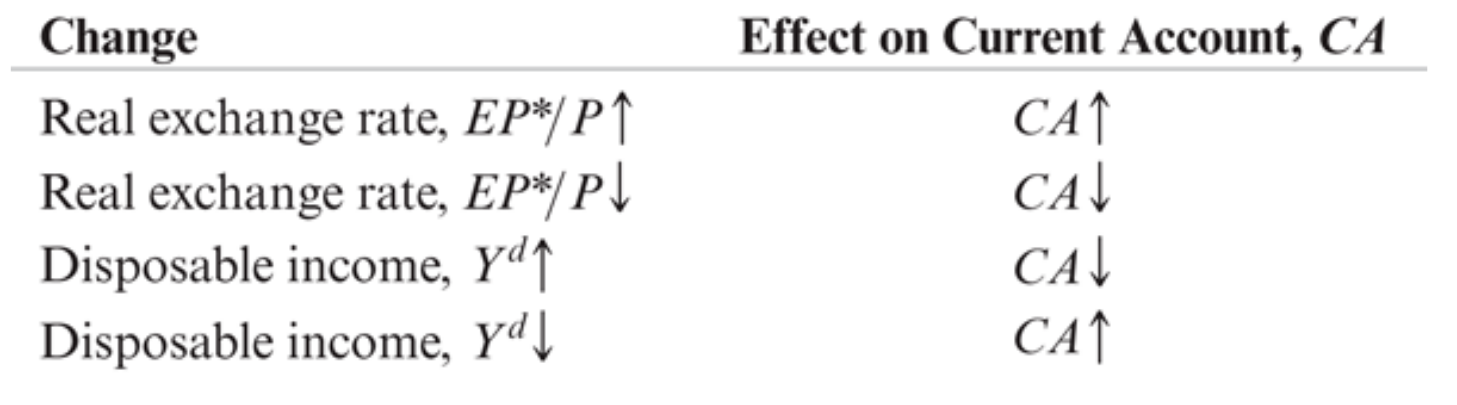
\includegraphics[scale=0.20]{ca_summary.png}
}

\begin{frame}{Components of aggregate demand}
        
        \begin{enumerate}
            \item Consumption is a function of national product, elasticity less than one
            \item Current account is a increasing function of real exchange rate, and decreasing function of disposable income 
        \end{enumerate}
\end{frame}

\frame{% how to print
\frametitle{Determinants of Aggregate Demand in the Short Run: $G, I$}
\begin{itemize}
\item For entire chapter, assume that $I$ spending on investment is fixed
\begin{itemize}
    \item In particular, assume that product not used as consumption spent on imports
\end{itemize}
\item Government spending will be treated later
\item For now let $G$ be fixed
\end{itemize}
}

\begin{frame}{Components of aggregate demand}
        
        \begin{enumerate}
            \item Consumption is a function of national product, elasticity less than one
            \item Current account is a increasing function of real exchange rate, and decreasing function of disposable income 
            \item Investment spending is fixed
            \item Government spending is fixed
        \end{enumerate}
\end{frame}

\frame{% how to print
\frametitle{Determinants of Aggregate Demand in the Short Run}
Aggregate demand:
\begin{center}
$D=C+I+G+CA$
\end{center}
Plug in components as functions
\begin{center}
$D = C\left(Y - T\right) + I + G + CA\left(\frac{E P^{*}}{P}, Y -T\right)$
\end{center}
or 
\begin{center}
$D = D\left(\frac{E P^{*}}{P}, Y - T, I, G\right)$
\end{center}
$I$ and $G$ are set outside our model

$D$ is increasing in real exchange rate

What happens to $D$ after a rise in disposable income?
}

\frame{% how to print
    \frametitle{Aggregate demand}
    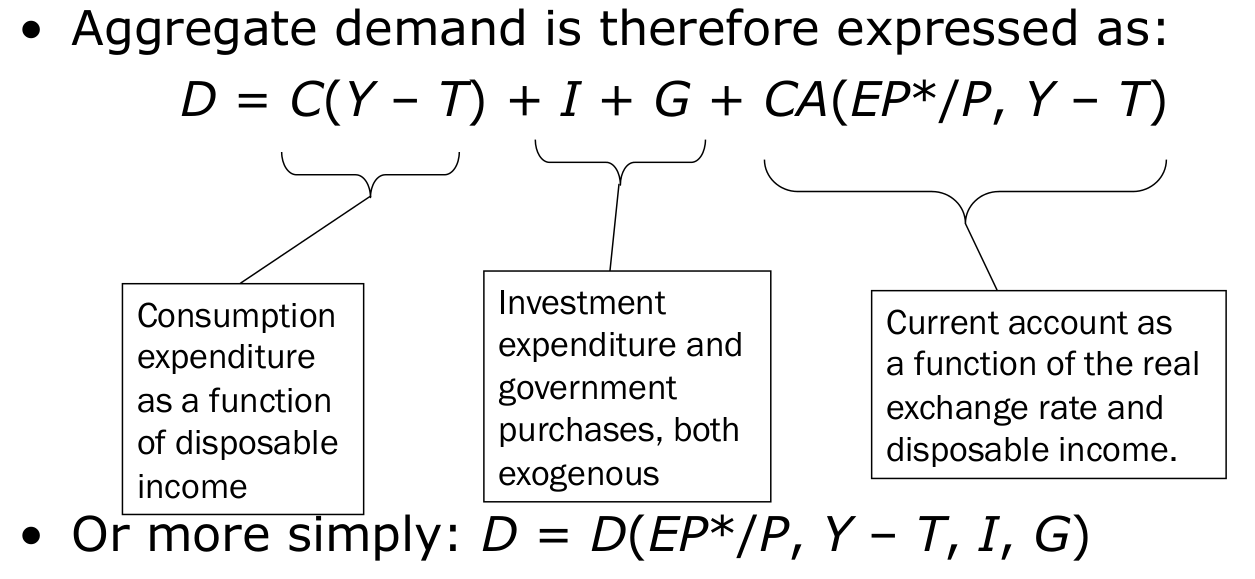
\includegraphics[scale=0.25]{ag_demand_eq.png}
}

\frame{
\frametitle{Determinants of Aggregate Demand in the Short Run}
Two effects:
\begin{enumerate}
\item \textbf{Real exchange rate:} $\frac{E P^{*}}{P} \Uparrow \Rightarrow CA \Uparrow \Rightarrow D \Uparrow$
\item \textbf{Disposable income:} $ \left(Y-T\right)\Uparrow \Rightarrow C \Uparrow, CA \Downarrow$
\end{enumerate}
\begin{itemize}
\item Assume that if consumers get one more dollar, spend most of it on domestic production rather than foreign $\Rightarrow D \Uparrow$
\end{itemize}
}

\frame{% how to print
    \frametitle{Aggregate demand}
    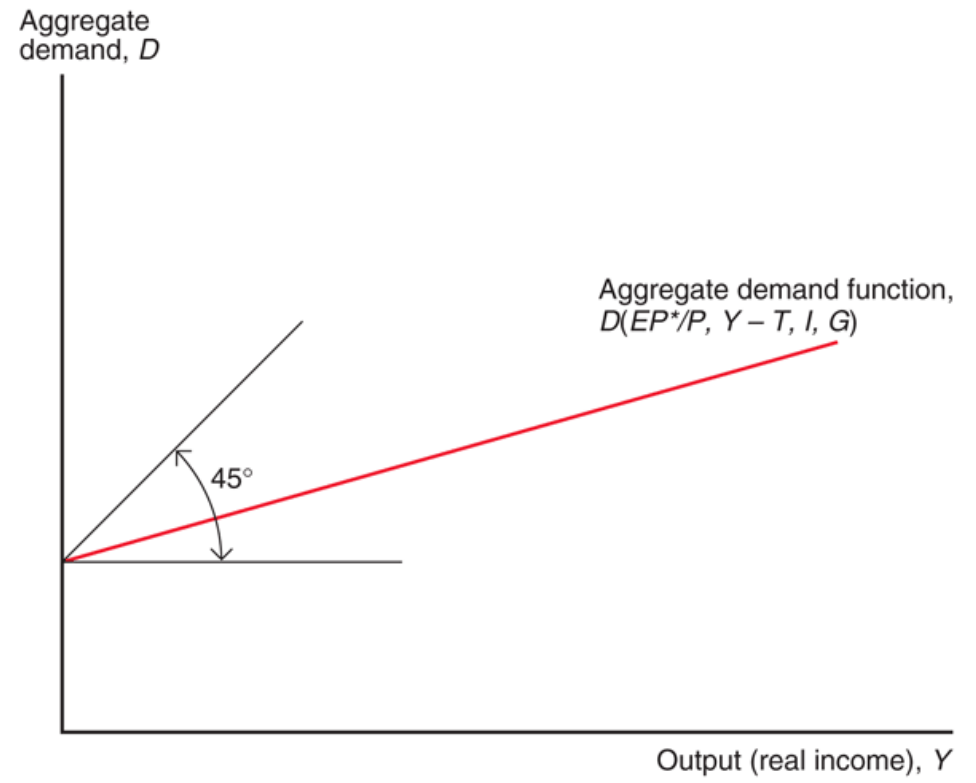
\includegraphics[scale=0.25]{ag_demand.png}
}

\frame{
\frametitle{Short Run Equilibrium for Aggregate Demand and Output}
\begin{itemize}
    \item Equilibrium is achieved when the value of income from production (output) Y equals the value of aggregate demand D.
    \begin{center}
    $Y= D\left(\frac{E P^{*}}{P}, Y - T, I, G\right)$
    \end{center}
    \item Short run, because we don't allow money prices of goods to adjust
    \item Later in chapter, we will show how demand moves towards long run equilibrium
\end{itemize}
}


\frame{
\frametitle{The Determination of Output in the Short Run}
\begin{figure}
	\centering
		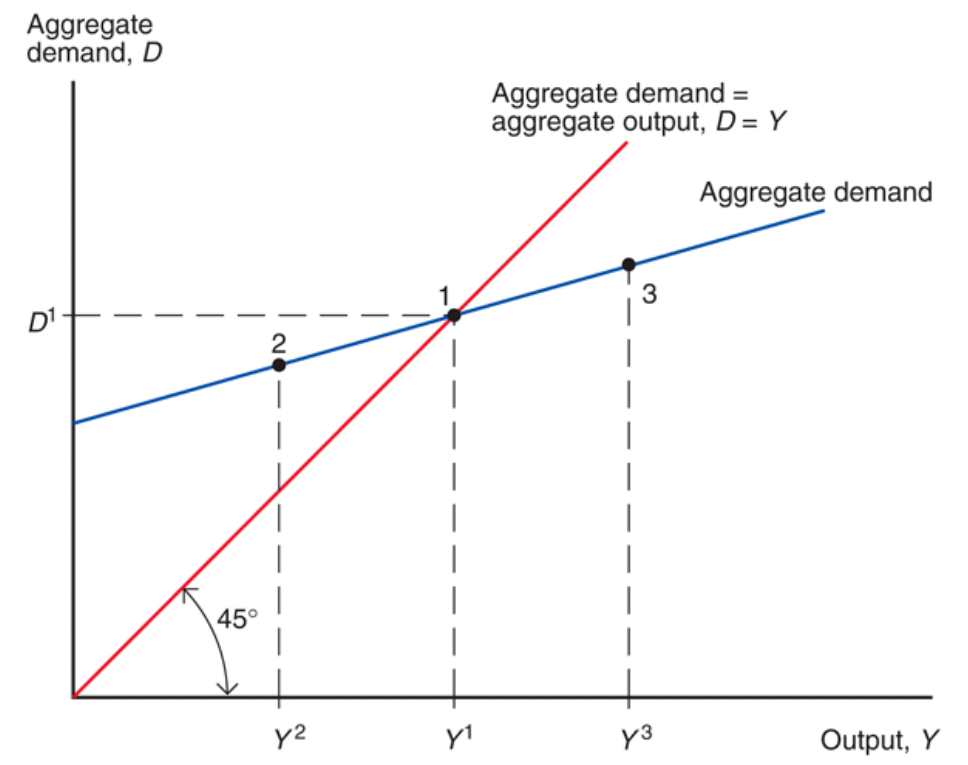
\includegraphics[scale=0.25]{short_run_eq.png}
	\label{fig:11}
\end{figure}
}


\frame{
\frametitle{DD Schedule}
\begin{itemize}
\item The DD Schedule is the relationship between exchange rates and output
\item Real depreciation of domestic currency increases demand for domestic goods
\item Production has to increase to meet demand 
\end{itemize}
}


\frame[plain]{
\frametitle{Output Effect of a Currency Depreciation with Fixed Output Prices}
\begin{figure}
	\centering
		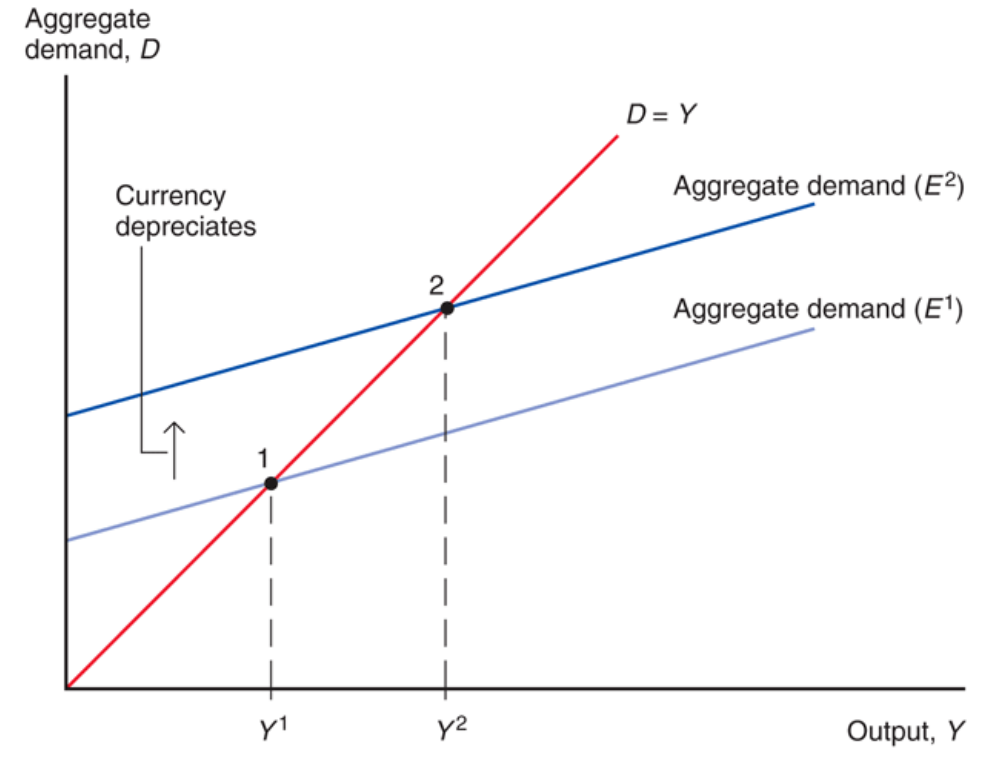
\includegraphics[scale=0.25]{demand_output.png}
\end{figure}
}

\frame{
\frametitle{DD Schedule}
\begin{itemize}
    \item Fix everything in aggregate demand except output $Y$ and nominal exchange rate $E$
    \item $DD$: Set of all $Y$ and $E$ at which the output market is in short run equilibrium 
\end{itemize} 
		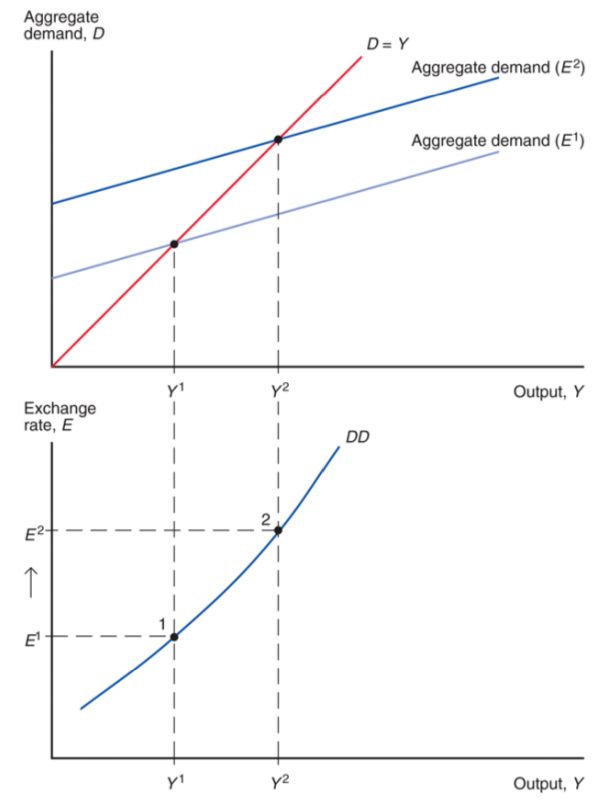
\includegraphics[scale=0.25]{dd_schedule.png}
}


\frame{
\frametitle{DD Schedule}
\begin{center}
    $Y= D\left(\frac{E P^{*}}{P}, Y - T, I, G\right)$
\end{center}
\begin{itemize}
    \item What causes changes in the $DD$ schedule?
    \begin{itemize}
        \item $G$: If government spending goes up, aggregate demand and output do too
    \end{itemize} 
\end{itemize}
}

\frame[plain]{
\frametitle{Government Demand and the Position of the DD Schedule}
\begin{figure}
	\centering
		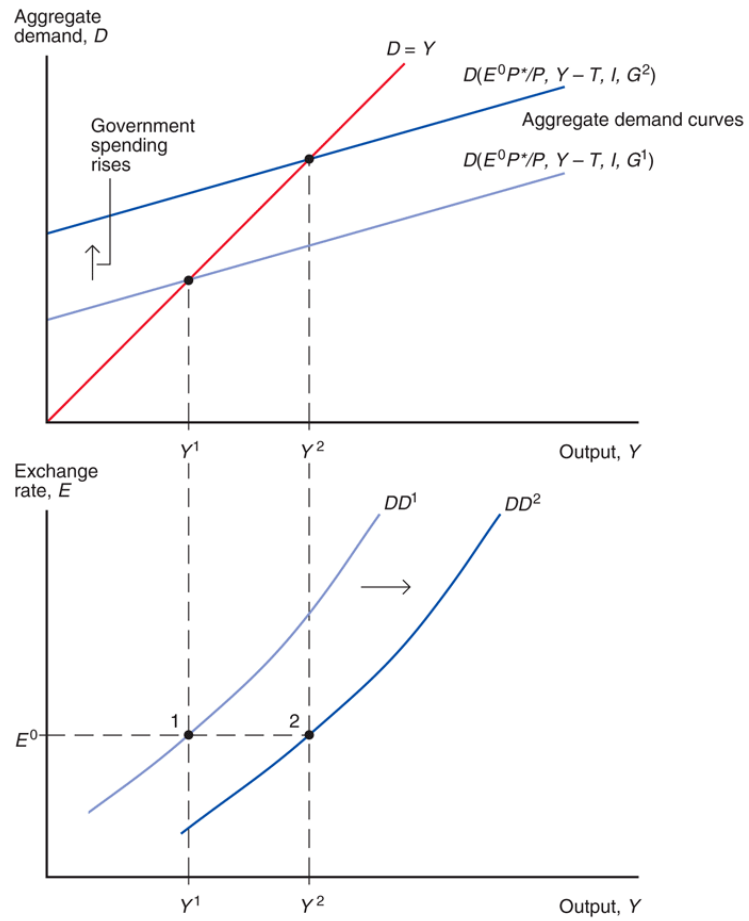
\includegraphics[scale=0.2]{goverment_demand_DD.png}
\end{figure}
}

\frame{
\frametitle{DD Schedule}
\begin{center}
    $Y= D\left(\frac{E P^{*}}{P}, Y - T, I, G\right)$
\end{center}
\begin{itemize}
    \item What else causes changes in the $DD$ schedule?
    \begin{itemize}
        \item $T$: if $T\Downarrow \Rightarrow C \Uparrow \Rightarrow D \& Y \Uparrow$
        \item $I$: if $I\Uparrow \Rightarrow D \& Y \Uparrow$ 
        \item $\frac{P}{P^{*}}$: if $\frac{P}{P^{*}} \Downarrow \Rightarrow D \& Y \Uparrow$
        \item $C$: if $C\Uparrow \Rightarrow D \& Y \Uparrow$
        \item demand of domestic goods with respect to the demand of foreign goods: $D \& Y \Uparrow$
    \end{itemize} 
\end{itemize}
}

\frame{
\frametitle{DD Schedule}
\begin{itemize}
    \item Moral of the story:
    \begin{itemize}
        \item Whatever causes an increase in aggregate demand causes a rightward shift of $DD$ curve 
    \end{itemize} 
\end{itemize}
}

\frame{
\frametitle{Pause}
\begin{itemize}
    \item So far:
    \begin{itemize}
        \item The $DD$ curve is the \emph{set} of possible output market equilibria
        \item That is every possible short-run equilibrium pair of $E$ and $Y$
    \end{itemize} 
    \item Discussion:
    \begin{itemize}
        \item For now $E$ (or real interest rate) and $Y$ output are the only endogenous objects
        \item Everything else is fixed
        \item Even then: Can't pin down a single equilibrium
    \end{itemize}
    \item Next:
    \begin{itemize}
        \item We need the sets of $E$ and $Y$ that put the asset market in short-run equilibrium
        \item DD curve slopes up, so don't be surprised taht our asset market curve will go down!
    \end{itemize}
\end{itemize}
}


\frame{
\frametitle{Short Run Equilibrium in Asset Markets}
Two sets of assets markets:
\begin{enumerate}
\item Foreign exchange markets 
\begin{center}
$R = R^{*}+ \frac{(E^{e} - E)}{E}$ 
\end{center}
\item Money market
\begin{center}
$\frac{M^{s}}{P}= L\left(R, Y\right) $
\end{center}
\end{enumerate}
Something we are used to!

BUT: Now we are going to fix everything but $Y$ and $E$
}


\frame[plain]{
\frametitle{Output and the Exchange Rate in Asset Market Equilibrium}
\begin{figure}
	\centering
		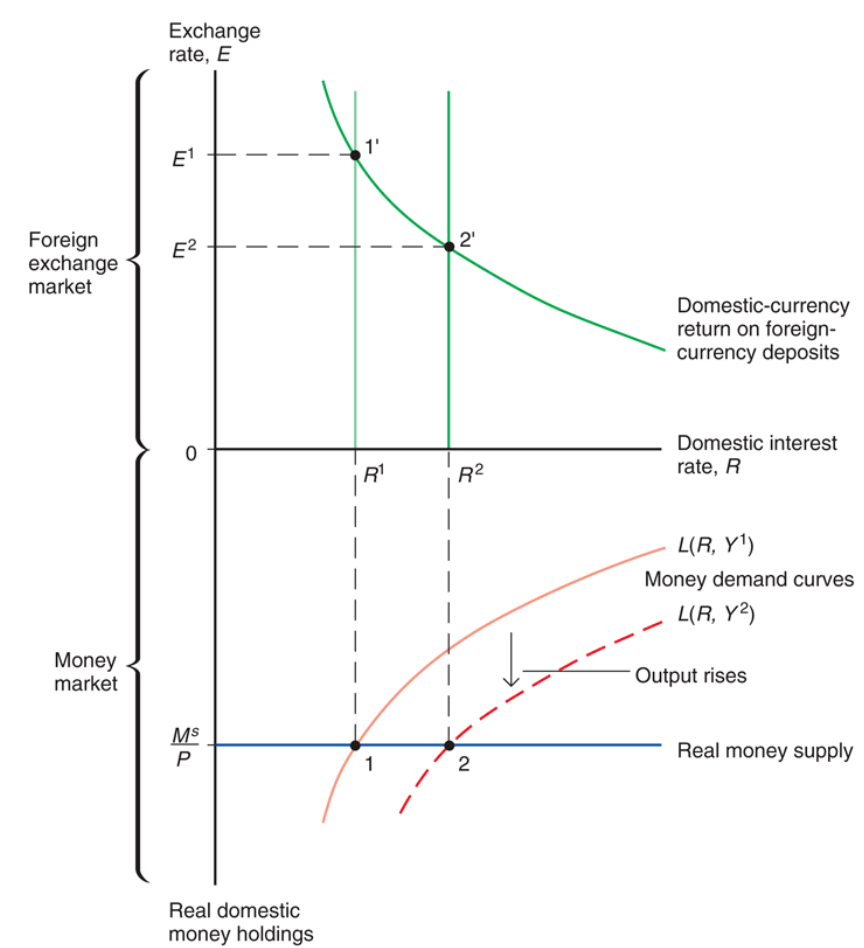
\includegraphics[scale=0.25]{asset_market_equilibrium.png}
	\label{fig:11}
\end{figure}
}


\frame{
\frametitle{Short Run Equilibrium in Asset Markets: AA Curve}
If $Y \Uparrow$:
\begin{enumerate}
\item $L\left(R, Y\right) \Uparrow$
\item $R \Uparrow$
\item $E \Downarrow$
\end{enumerate}
Output up, exchange rate down (appreciation)

How convenient, going to give us a downward sloping $AA$ curve!
}

\frame[plain]{
\frametitle{The AA Schedule}
\begin{figure}
	\centering
		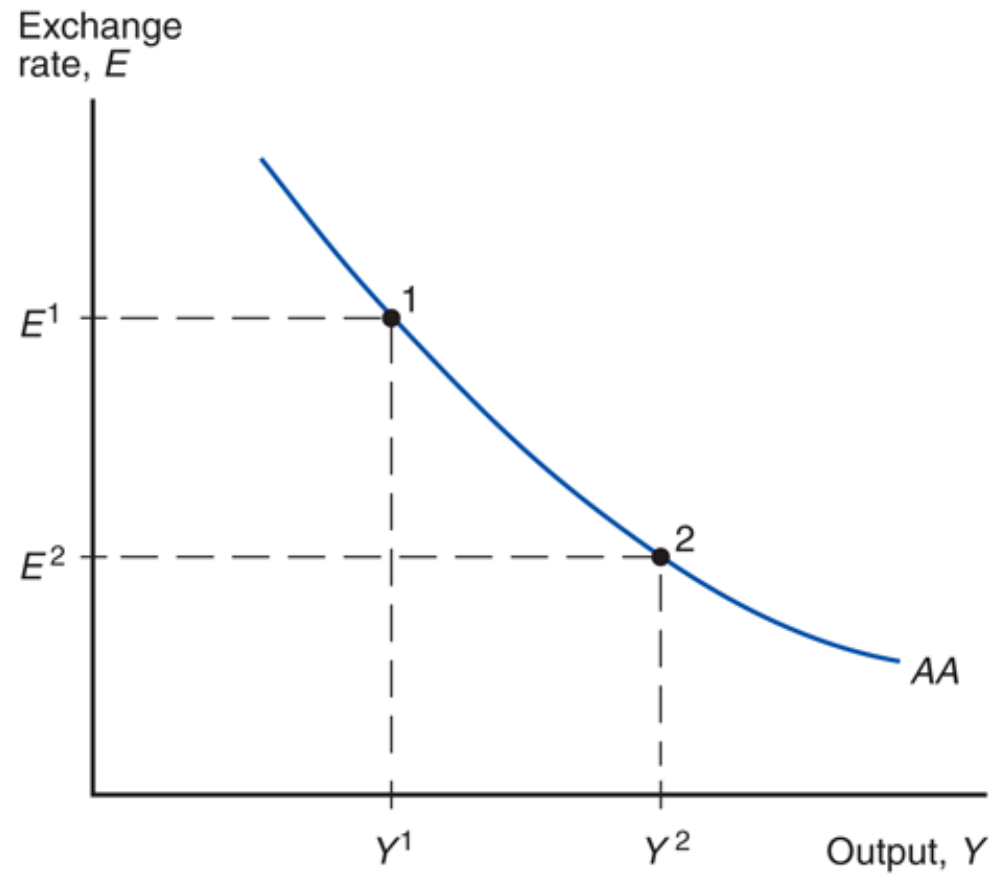
\includegraphics[scale=0.25]{AA_curve.png}
\end{figure}
}

\frame{
\frametitle{AA Schedule}
Money supply shift causes $AA$ to shift:
\begin{itemize}
\item $M^{s}$: if $M^{s}\Uparrow \Rightarrow R \Downarrow \Rightarrow E \Uparrow$: $AA$ shifts up.  
\end{itemize} 
}

\frame[plain]{
\frametitle{The AA Schedule: Increase in money}
\begin{figure}
	\centering
		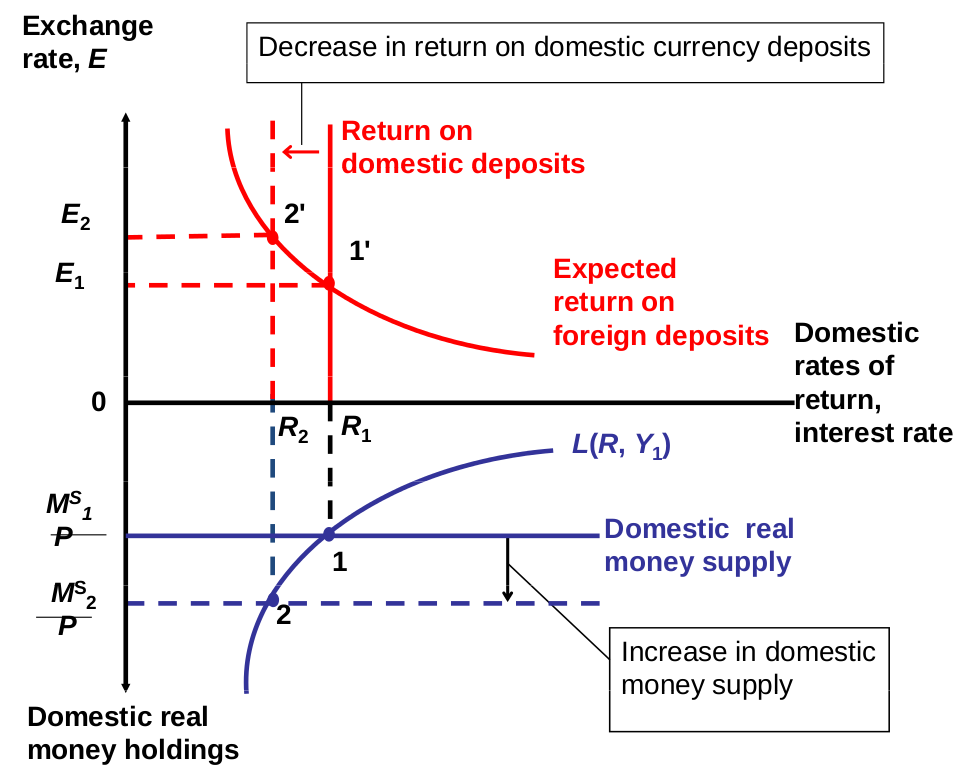
\includegraphics[scale=0.3]{AA_shift.png}
\end{figure}
}

\frame[plain]{
\frametitle{The AA Schedule: Increase in money}
\begin{figure}
	\centering
		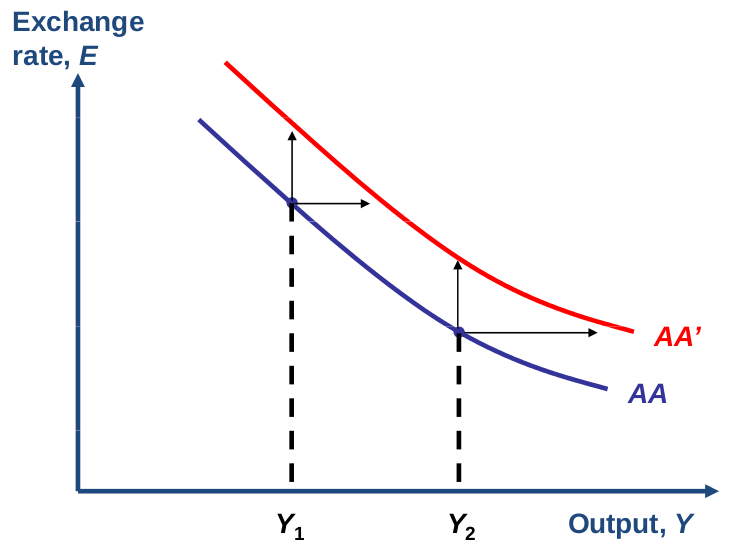
\includegraphics[scale=0.3]{AA_shift2.png}
\end{figure}
}

\frame{
\frametitle{AA Schedule}
Other things causing $AA$ to shift:
\begin{itemize}
\item $P$: if $P\Uparrow \Rightarrow \frac{M^{s}}{P} \Downarrow \Rightarrow R \Uparrow \Rightarrow E \Downarrow$: $AA$ shifts down.
\item $L\left(R,Y\right)$: if $L\left(R,Y\right)\Downarrow\Rightarrow$ more non-monetary assets $\Rightarrow E \Uparrow$: $AA$ shifts up.
\item $R^{*}$: if $R^{*}\Uparrow E \Uparrow$: $AA$ shifts up. 
\item $E^{e}$: if $E^{e}\Uparrow \Rightarrow AA \Uparrow$
\end{itemize} 
}
 
\begin{frame}{Pause}
    \begin{itemize}
        \item Fix everything but $Y$ and $E$
        \item We have set of equilibria in output market (Output supply equals aggregate demand)
        \item We have set of equilibria in asset market
        \item Now let us find the point where both the output and asset market are in equilibrium
    \end{itemize}
\end{frame}

\frame{
\frametitle{Short Run Equilibrium}
A short run equilibrium means $E$ and $Y$ such that:
\begin{enumerate}
\item equilibrium in the output markets holds (DD): $D=Y$
\item equilibrium in the foreign exchange markets holds (AA): $R = R^{*}+ \frac{(E^{e} - E)}{E}$ 
\item equilibrium in the money market holds: $M^{s}=M^{d}$
\end{enumerate}
}

\frame{
\frametitle{Short-Run Equilibrium: The Intersection of DD and AA}
\begin{itemize}
    \item Begining to think everything in undergrad econ is the same picture
    \item Just change the labels
\end{itemize}
\begin{figure}
	\centering
		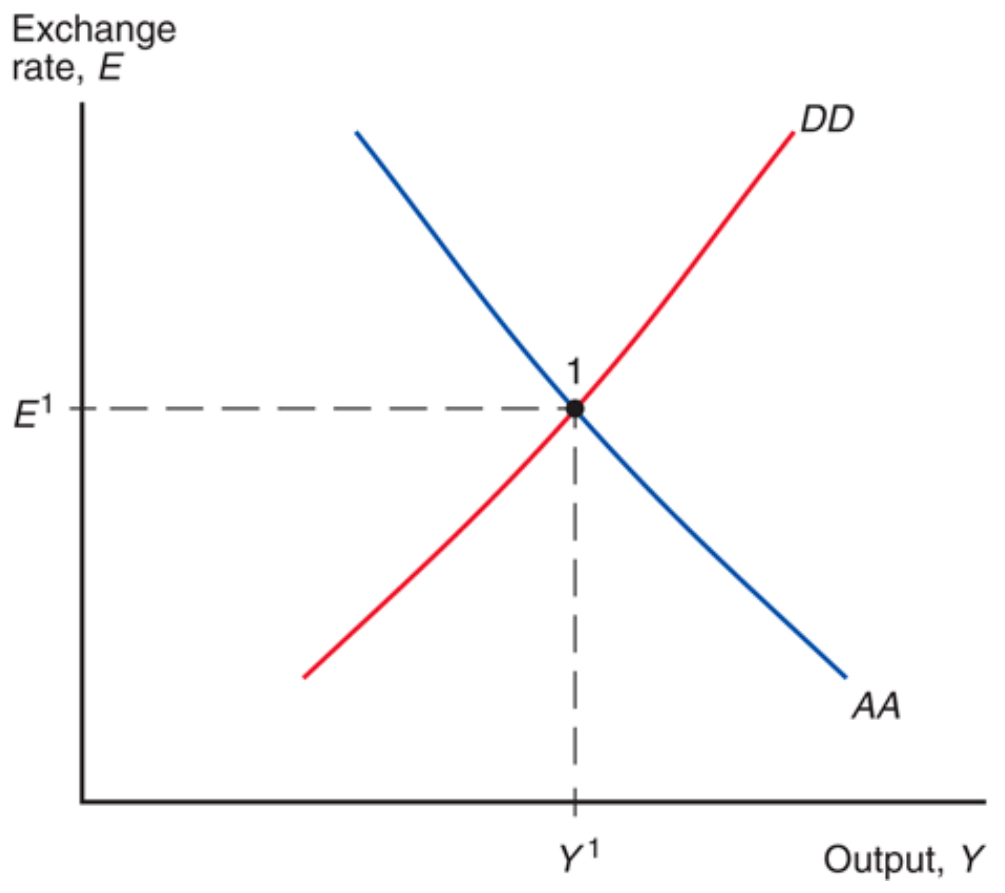
\includegraphics[scale=0.20]{full_short_run_eq.png}
\end{figure}
}


\frame[plain]{
\frametitle{How the Economy Reaches Its Short-Run Equilibrium}
\begin{itemize}
    \item Drop to $3$ to maintain interet rate parity
    \item Travel to $1$ as excess demand firms to increase production, which increases real money demand, which raises interest rate, which causes appreciation of currency
\end{itemize}
\begin{figure}
	\centering
		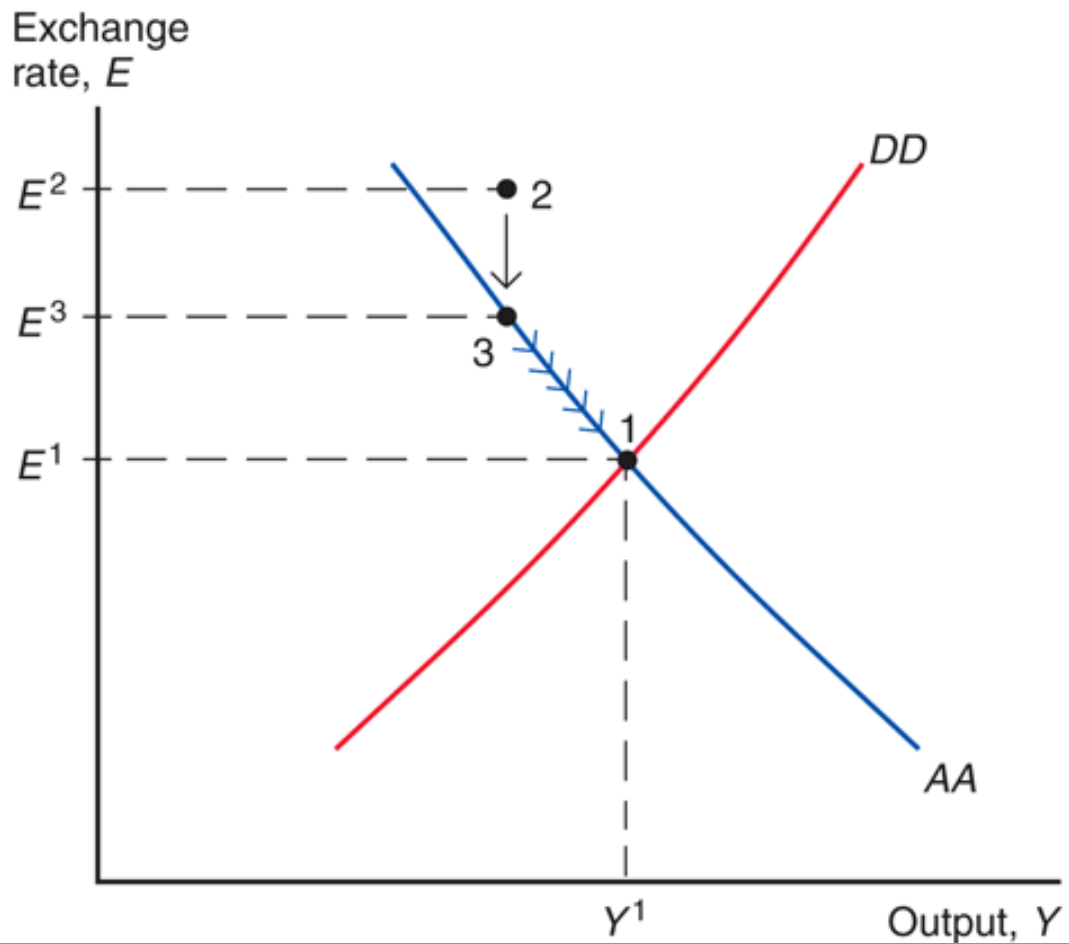
\includegraphics[scale=0.17]{path_to_eq.png}
\end{figure}
}

\begin{frame}{Pause}
    \begin{itemize}
        \item Fix everything but $Y$ and $E$
        \item We have set of equilibria in output market (Output supply equals aggregate demand)
        \item We have set of equilibria in asset market
        \item We have the point where both markets are in equilibrium 
        \item If only $Y$ and $E$ are allowed to adjust in the short-run, our model is powerful
        \item We can analyze the effects of goverment policy ($M$ and $G$)
    \end{itemize}
\end{frame}

\frame{
\frametitle{Temporary Changes in Monetary and Fiscal Policy}
\begin{itemize}
\item \textbf{Monetary policy:} the central bank influences the supply of monetary assets (AA) 
\item \textbf{Fiscal policy:} governments influence the amount of government purchases and taxes (DD)
\end{itemize}
Suppose that the policies are going to be undone after a short period
}

\frame{
\frametitle{Temporary Monetary Policy}
\begin{itemize}
\item if $M^{s} \Uparrow \Rightarrow R \Downarrow E \Uparrow$
\item $AA$ shifts up
\end{itemize}
}

\frame{
\frametitle{Temporary Changes in Monetary and Fiscal Policy}
\begin{figure}
	\centering
		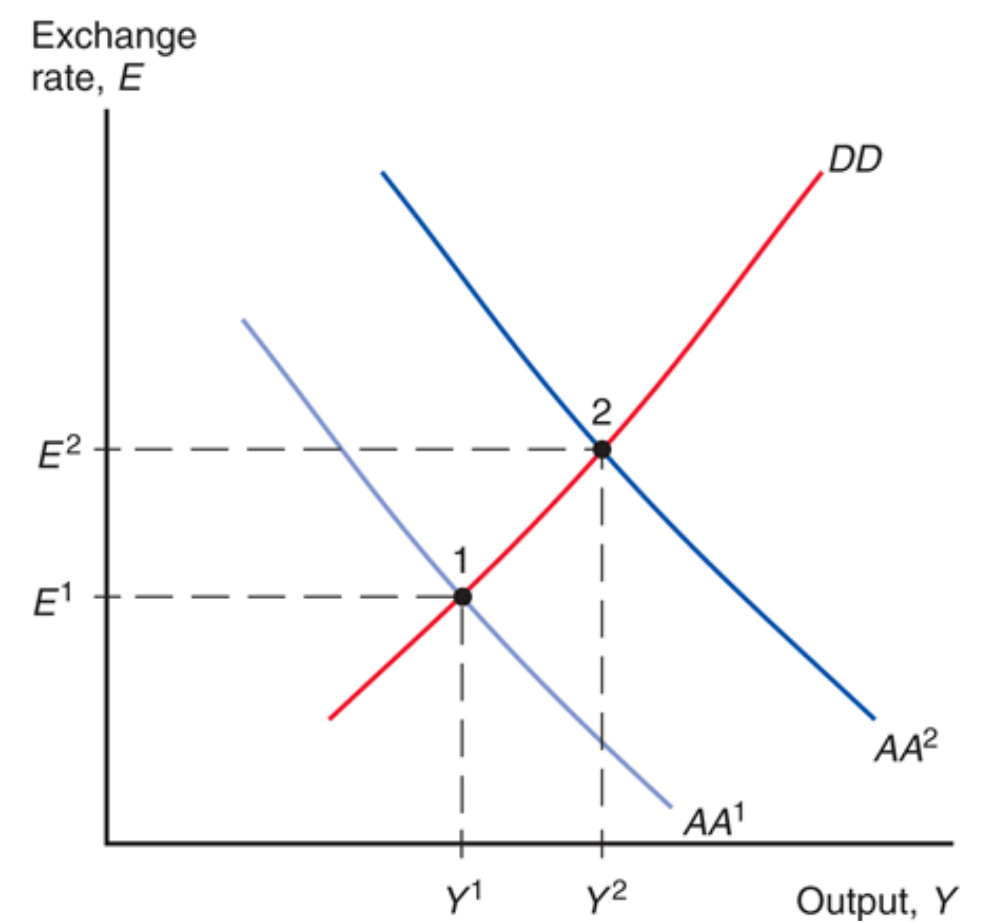
\includegraphics[scale=0.25]{money_supply_increase.png}
	\label{fig:11}
\end{figure}
}

\frame{
\frametitle{Temporary Fiscal Policy}
Government decides to build a space shuttle
\begin{itemize}
\item if $G \Uparrow$ (or $T \Downarrow$) $\Rightarrow D \& Y \Uparrow$
\item $DD$ shifts down
\item $Y \Uparrow \Rightarrow L\left(Y,R\right) \Uparrow \Rightarrow R \Uparrow$
\item $E \Downarrow$
\end{itemize}
}

\frame{
\frametitle{Effects of a Temporary Fiscal Expansion}
\begin{figure}
	\centering
		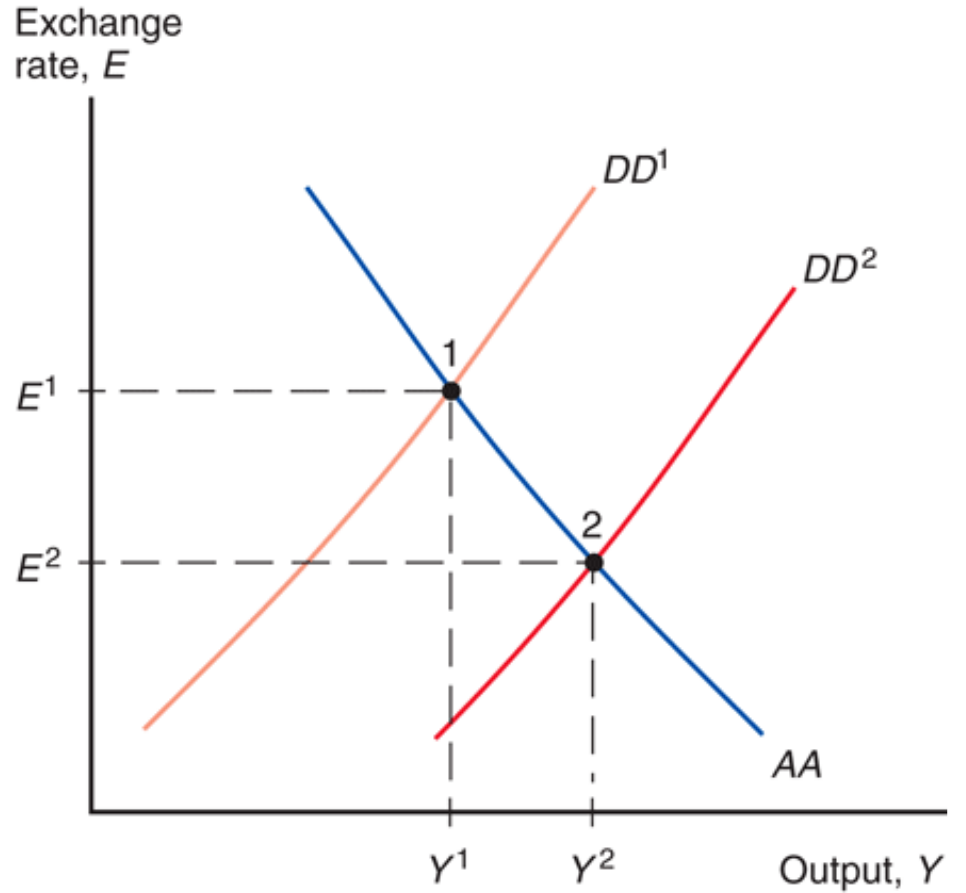
\includegraphics[scale=0.25]{fiscal_expansion.png}
\end{figure}
}

\frame{
\frametitle{Policies to Maintain Full Employment}
\begin{itemize}
    \item How might governments use these policy tools?
    \item Suppose there is a temporary shift of consumer taste away from domestic product
    \item This will shift $DD$ up, resulting in unemployment (factors same, drop in $Y$)
    \item Central bank can increase money supply
\end{itemize}
}

\frame[plain]{
\frametitle{Maintaining Full Employment After a Temporary Fall in World Demand for Domestic Products}
\begin{figure}
	\centering
		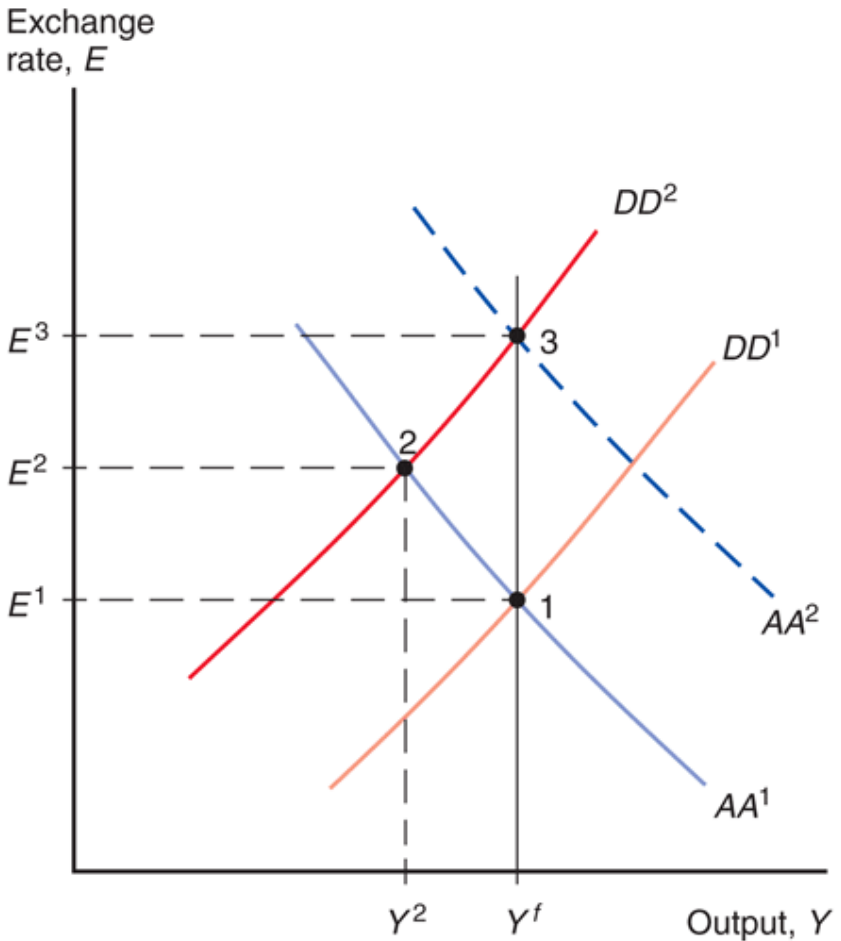
\includegraphics[scale=0.20]{monetary_policy.png}
\end{figure}
}

\frame{
\frametitle{Policies to Maintain Full Employment}
\begin{itemize}
    \item How might governments use these policy tools?
    \item Suppose people suddenly demand more money 
    \item This will shift $AA$ down, resulting in unemployment 
    \item Government can demand more stuff, raising $DD$ 
\end{itemize}
}

\frame[plain]{
\frametitle{Policies to Maintain Full Employment After a Money Demand Increase}
\begin{figure}
	\centering
		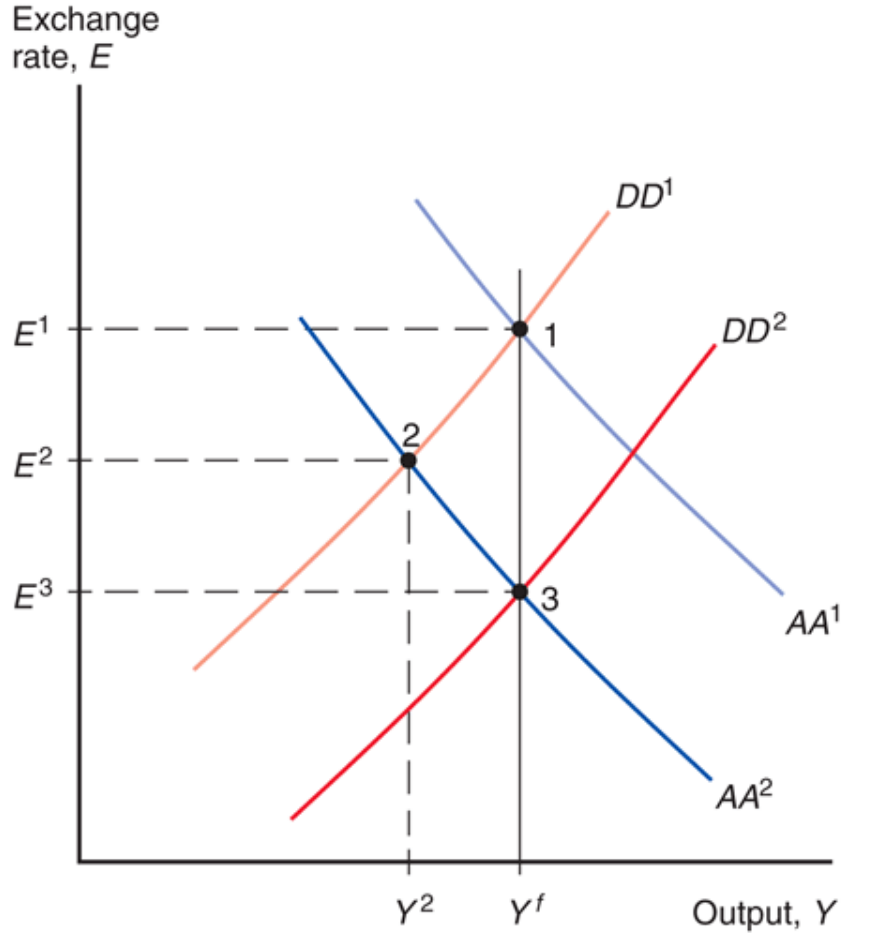
\includegraphics[scale=0.2]{fiscal_policy.png}
\end{figure}
}

\frame{
\frametitle{Policies to Maintain Full Employment}
Policies to maintain full employment are difficult to implement:
\begin{itemize}
\item inflation bias
\begin{itemize}
    \item Government is expected print money to expand output and win an election
    \item Workers anticipate inflation, ask for higher wages 
    \item Costs rise leading to less output and unemployment 
    \item Government needs monetary policy just to return to baseline output
\end{itemize}
\item Difficult to tell if problem is in the asset or output market 
\begin{itemize}
    \item Which tool?
\end{itemize}
\item Policy lag
\item Monetary policy much faster
\begin{itemize}
    \item Government may use it even when fiscal policy is more appropriate
\end{itemize}
\item Ricardian equivalence
\end{itemize}
}

\begin{frame}{Pause}

    \begin{itemize}
        \item We have seen how governments might use temporary policy instruments
        \item Next let us look at permanent policy changes
        \begin{itemize}
            \item A permanent expansion of the money supply
            \item A permanent increase in government demand
        \end{itemize}
        \end{itemize}
\end{frame}

\frame{
\frametitle{Permanent Changes in Monetary Policy}
\begin{itemize}
    \item Permanent money expansion: Short-Run
    \begin{itemize}
        \item Short run: Lower interest rate $\rightarrow$ depreciation
        \item Short run: Expected future depreciation $\rightarrow$ more depreciation
        \item AA curve shifts up more than in the temporary monetary case 
    \end{itemize}
\end{itemize}
}


\frame[plain]{
\frametitle{Short-Run Effects of a Permanent Increase in the Money Supply}
\begin{figure}
	\centering
		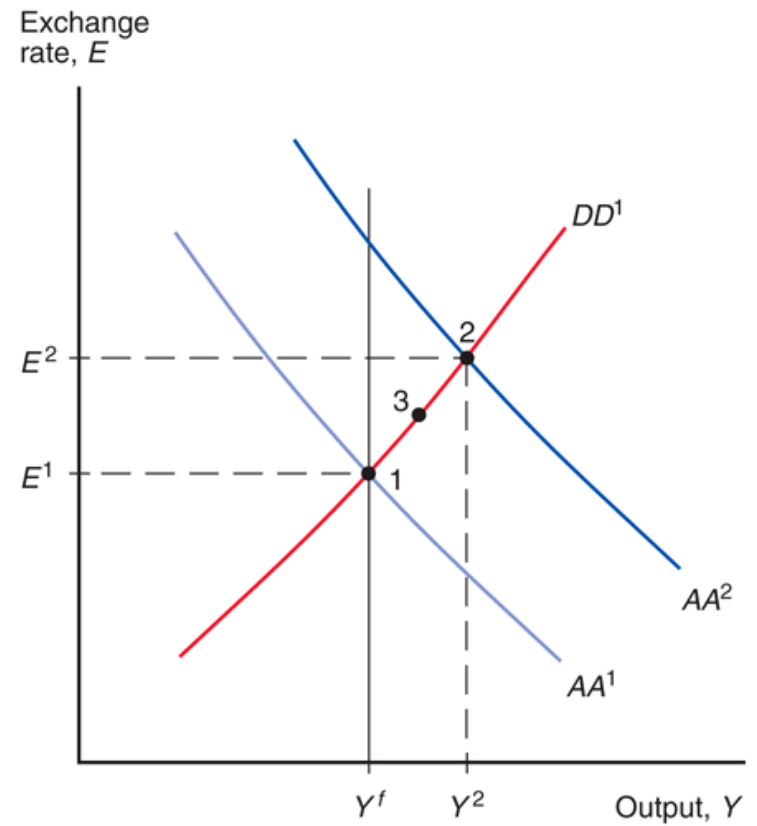
\includegraphics[scale=0.25]{short_run_perm_money.png}
	\label{fig:11}
\end{figure}
}

\frame{
\frametitle{Permanent Changes in Monetary Policy}
\begin{itemize}
    \item Permanent money expansion: Long-run
    \begin{itemize}
        \item Long-run: factors are running overtime to meet production, rising costs, rising prices
        \item Long-run: Rising prices encourage imports, shifting $DD$ in
        \item Long-run: Rising prices lower real money supply, shifting $AA$ in
        \item Reach equilibrium at long-run production level (full-employment)
    \end{itemize}
\end{itemize}
}

\frame[plain]{
\frametitle{Permanent Changes in Monetary Policy}
\begin{figure}
	\centering
		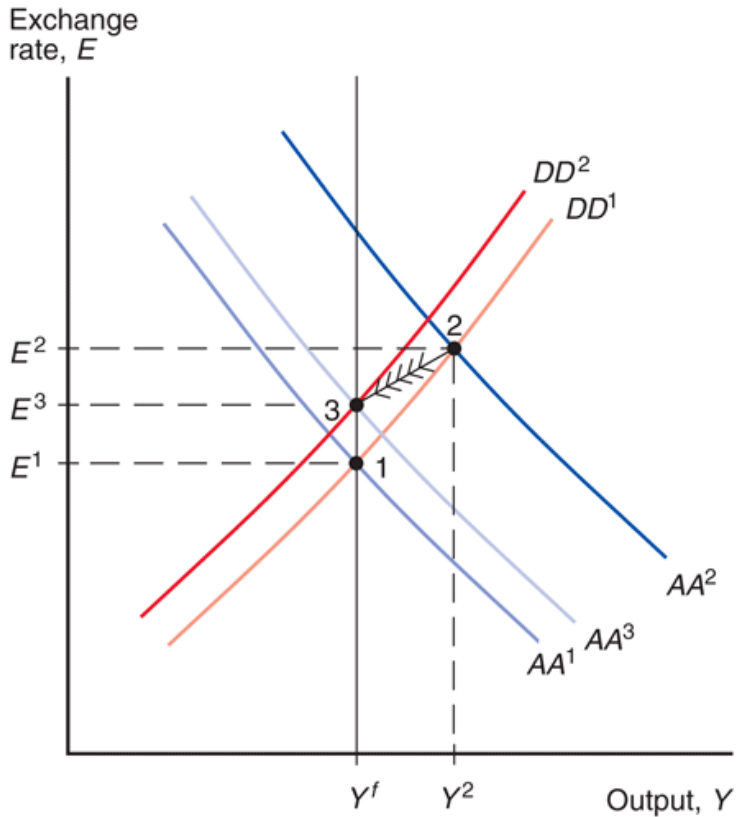
\includegraphics[scale=0.2]{long_run_perm_money.png}
\end{figure}
}

\frame{
\frametitle{Effects of Permanent Changes in Fiscal Policy}
If $G \Uparrow$ or $T \Downarrow$
\begin{itemize}
    \item Two effects:
    \begin{enumerate}
        \item Increase aggregate demand (shift out $DD$ curve)
        \item Causes expectations of a future exchange rate appreciation (shift in $AA$)
    \end{enumerate}
    \item An permanent increase in government purchases is exactly offset by reduction in exports due to currency appreciation
\end{itemize}
}


\frame[plain]{
\frametitle{Fig. 17-16: Effects of a Permanent Fiscal Expansion}
\begin{figure}
	\centering
		\includegraphics[width=0.90\textwidth]{diciotto.pdf}
	\label{fig:11}
\end{figure}
}
% 
% \Section{Chapter 17. Macroeconomic Policies and the Current Account (XX curve)}
% 
% \frame{
% \frametitle{Macroeconomic Policies and the Current Account}
% \begin{itemize}
% \item XX curve: combinations of output and exchange rates at which the current account is at its desired level. 
% \item if $Y \Uparrow \Rightarrow CA \Downarrow$
% \item XX curve slopes upward but is flatter than the DD curve
% \end{itemize}
% }
% 
% \frame[plain]{
% \frametitle{Fig. 17-17: How Macroeconomic Policies Affect the Current Account}
% \begin{figure}
% 	\centering
% 		\includegraphics[width=0.90\textwidth]{diciannove.pdf}
% 	\label{fig:11}
% \end{figure}
% }
% 
% \frame[plain]{
% \frametitle{Fig. 17-17: How Macroeconomic Policies Affect the Current Account}
% \begin{figure}
% 	\centering
% 		\includegraphics[width=0.90\textwidth]{venti.pdf}
% 	\label{fig:11}
% \end{figure}
% }
% 
% 
% \frame[plain]{
% \frametitle{Fig. 17-18: The J-Curve}
% \begin{figure}
% 	\centering
% 		\includegraphics[width=0.90\textwidth]{ventidue.pdf}
% 	\label{fig:11}
% \end{figure}
% }
% 
% \begin{frame}{Overall trade review}
% 
% \begin{tikzpicture}
% \tikzset{scale=0.75,grow'=right,level distance=70pt}
% \tikzset{execute at begin node=\strut}
% \tikzset{every tree node/.style={anchor=base west}}
% 
% \Tree   [.Int\ Econ                     [.Trade     [.Theory    [.Comparative\ advantage ]
%                                                                 [.Factor\ endowments ]
%                                                                 [.Specific\ factors ]
%                                                                 [.Scale\ economies ]
%                                                                 [.Standard\ model ] ]
%                                                     [.Policy    [.Policy\ instruments ]
%                                                                 [.Political\ economy ] ] ]
%                                         [.Finance   [.Theory    [.Terminology\ and\ principles ]
%                                                                 [.Long-run\ exchange\ rates ] ]
%                                                     [.Policy    [.Short-run\ exchange\ rates ]
%                                                                 [.Coordination\ and\ Currency\ unions ] ] ] ]
% \end{tikzpicture}
% \end{frame}

\end{document}
